\chapter{Topics in String Theory: Strings and Black-Hole Entropy}

These notes follow Leonard Susskind's sixth lecture in the supplementary 2011 Winter Topics in String Theory track, with curation by LazyingArt LLC. The lecture asks a sharp question and keeps returning to it: if a black hole has entropy, then what microscopic objects are carrying that entropy? The answer is not presented here as a finished exact computation. Instead, the lecture assembles the simplest string-theoretic picture that gets the scaling right, shows why a long excited string and a black hole can be connected by varying the coupling, and leaves the final algebraic payoff for the next lecture.

\section{Entropy and the Microscopic Question}

Susskind begins by lowering the level of abstraction. To say that a system has a large entropy is to say that it contains many microscopic degrees of freedom which are too small and too numerous to keep track of individually. In that sense entropy is a measure of hidden information.

The analogy is an ordinary fluid. Fluid dynamics is a coarse-grained theory: it describes velocity, density, and macroscopic flow, but it does not say what the microscopic constituents of the fluid are. Thermodynamics then tells us that the fluid has entropy, and that becomes evidence for a deeper microscopic structure. The entropy does not itself identify the atoms, but it tells us that some such microscopic structure must exist.

The same logic is then applied to gravity, and in particular to black holes. Bekenstein-Hawking entropy tells us that a black hole carries an enormous amount of hidden information, and because that entropy is proportional to the area, one is led to ask what microscopic things are somehow living on, or associated with, the horizon. General relativity by itself gives no clear microscopic answer. String theory, in the lecture's framework, offers a candidate answer. Susskind emphasizes from the outset that the argument will be qualitative and order-of-magnitude in character, but that it will nevertheless reveal the correct structure of the problem.

\section{Planck Scale, String Scale, and the Coupling}

The lecture then pauses to collect the basic scales and constants. On the gravity side, the distinguished length is the Planck length,
\begin{equation}
\ell_p=\sqrt{\frac{G_N\hbar}{c^3}}.
\end{equation}
Susskind quickly moves to units in which
\begin{equation}
\hbar=c=1,
\end{equation}
so that Newton's constant becomes the Planck area:
\begin{equation}
\ell_p^2=G_N.
\end{equation}
In these units \(G_N\) has dimensions of area, and this is precisely why black-hole entropy is naturally measured as horizon area in Planck units.

String theory comes with its own length scale, the string length \(\ell_s\). Rather than defining it formally, the lecture motivates it physically: a heated string wiggles, but those wiggles do not continue to arbitrarily short scales. There is a characteristic scale of stringy oscillation, and that is the string length.

The third ingredient is the string coupling. In the lecture it is introduced operationally as the amplitude, or probability-like control parameter, for a string to split when it crosses itself. In cleaned notation it is best denoted by \(g_s\). Susskind also interprets it as the analogue of electric charge in electrodynamics: if a charged particle emits a photon with amplitude \(e\), then a string emits a small string with amplitude \(g_s\). That small emitted string is, in particular, a graviton.

The lecture assumes \(g_s\) to be small. This is not yet the main argument, but it immediately implies a useful hierarchy: if \(g_s\ll 1\), then the Planck scale is smaller than the string scale. The black-hole/string comparison will be carried out with this hierarchy in mind.

\section{From Photon Exchange to Graviton Exchange}

Before writing any entropy formulas, Susskind inserts a diagrammatic bridge. Electromagnetic forces are first recalled in the familiar language of Feynman diagrams: one charged particle emits a photon, another absorbs it, and the interaction strength carries one factor of the charge from emission and one from absorption. At the level of scaling,
\begin{equation}
F_{\mathrm{EM}}\propto e^2.
\end{equation}
The lecture immediately warns that this picture should not be taken too literally as one particle simply shooting a photon at another, but it is a useful guide to the structure of the interaction.

\begin{figure}[htbp]
\centering

\includegraphics[width=0.62\textwidth]{lecture_06_figure_03.png}
\caption{Photon-exchange Feynman sketch on the board. The irregular looped residue above the main exchange diagram belongs to earlier board work and is not part of the reconstructed argument.}
\end{figure}

\begin{figure}[htbp]
\centering
\begin{tikzpicture}[scale=1.0]
\draw[line width=0.8pt] (0,0) -- (0,3.2);
\draw[line width=0.8pt] (4.8,0) -- (4.8,3.2);
\draw[line width=0.8pt] plot[smooth] coordinates
{(0,1.55) (0.6,1.78) (1.2,1.30) (1.8,1.82) (2.4,1.28) (3.0,1.80) (3.6,1.32) (4.2,1.74) (4.8,1.55)};
\end{tikzpicture}
\caption{Clean reconstruction of the exchanged-photon sketch used to motivate the interaction law.}
\end{figure}

The gravitational version is then obtained by analogy. If everything is made of strings, then two massive objects interact by exchanging a graviton. The emission amplitude is proportional to \(g_s\), and the absorption amplitude is proportional to \(g_s\) again, so the interaction strength scales as
\begin{equation}
F_{\mathrm{grav}}\propto g_s^2.
\end{equation}
But this is not yet Newton's constant: \(g_s\) is dimensionless, whereas \(G_N\) has dimensions of length squared. The only available length scale in the string description is \(\ell_s\), so dimensional analysis forces
\begin{equation}
G_N\sim g_s^2 \ell_s^2.
\end{equation}
Using \(\ell_p^2=G_N\), one obtains the basic relation
\begin{equation}
\ell_p=g_s\ell_s.
\end{equation}
This is one of the lecture's central formulas. It tells us how the gravitational scale is generated from the intrinsic string scale together with the strength of string interactions.

\section{Black-Hole Entropy and the Entropy of a Long String}

Once the scales are in place, the lecture turns to entropy formulas. The point is not to present two unrelated facts, but to place them side by side and then ask why they almost, but not quite, line up.

\subsection{Black-hole entropy}

Ignoring numerical constants such as the familiar factor of \(1/4\), the lecture writes the Bekenstein-Hawking entropy as
\begin{equation}
S_{BH}\sim \frac{A}{G_N}\sim \frac{A}{\ell_p^2}.
\end{equation}
This is the statement that the horizon area is being counted in Planck units.

The same formula can be rewritten in terms of the mass. Since the Schwarzschild radius is
\begin{equation}
R_s=2MG_N,
\end{equation}
and the horizon area scales as \(A\sim R_s^2\), one gets
\begin{align}
A &\sim R_s^2 \sim (MG_N)^2,\\
S_{BH} &\sim \frac{A}{G_N}\sim \frac{M^2G_N^2}{G_N}\sim M^2G_N\sim M^2\ell_p^2.
\end{align}

\paragraph{Worked derivation.}
At the level of scaling used throughout the lecture:
\begin{enumerate}
\item \(S_{BH}\sim A/G_N\).
\item \(A\sim R_s^2\).
\item \(R_s\sim MG_N\), after dropping the factor of \(2\).
\item Hence \(A\sim M^2G_N^2\).
\item Therefore \(S_{BH}\sim M^2G_N\sim M^2\ell_p^2\).
\end{enumerate}

\subsection{The entropy of a long excited string}

The lecture then deliberately changes tone. Instead of starting from a black hole, Susskind starts from a tiny string and pumps a great deal of energy into it. A highly excited string does not look like a neat oscillating loop; it looks like a tangled mess, more like an overtwisted fishing reel than a clean geometric object. Such tangled configurations should have entropy, because there are many ways to make a large jumbled string that look macroscopically alike.

To count this entropy, the lecture introduces a crude lattice model. Space is replaced by a lattice, and a string is modeled as a connected chain of links. The size of each link is taken to be the string length \(\ell_s\). In a two-dimensional toy lattice, each step has four possible continuations, even allowing the path to reverse. Thus a string with \(n\) links has a number of states of order
\begin{equation}
\Omega_{\text{string}}\sim 4^n.
\end{equation}
Entropy is the logarithm of the number of macroscopically indistinguishable states, so
\begin{equation}
S_{st}\sim \log \Omega_{\text{string}}\sim n\log 4\sim n.
\end{equation}
If \(L\) denotes the total length of the string measured by following it along the curve, then
\begin{equation}
n=\frac{L}{\ell_s},
\end{equation}
and therefore
\begin{equation}
S_{st}\sim \frac{L}{\ell_s}.
\end{equation}

The lecture then converts this into a mass formula. In the units \(\hbar=c=1\), mass scales as inverse length, so a single lattice link has mass
\begin{equation}
m_{\text{link}}\sim \frac{1}{\ell_s}.
\end{equation}
A string with \(n\) links therefore has total mass
\begin{equation}
M\sim \frac{n}{\ell_s}\sim \frac{L}{\ell_s^2}.
\end{equation}
Equivalently,
\begin{equation}
L\sim M\ell_s^2.
\end{equation}
Substituting this back into the entropy formula gives
\begin{equation}
S_{st}\sim M\ell_s.
\end{equation}

\paragraph{Worked derivation.}
The lattice argument can be summarized exactly in the lecture's spirit:
\begin{enumerate}
\item Model the excited string as a connected chain of \(n\) links of size \(\ell_s\).
\item Count states as \(\Omega\sim 4^n\) in the two-dimensional toy model.
\item Take the logarithm: \(S_{st}\sim n\).
\item Use \(n=L/\ell_s\) to obtain \(S_{st}\sim L/\ell_s\).
\item Use \(m_{\text{link}}\sim 1/\ell_s\), hence \(M\sim n/\ell_s\sim L/\ell_s^2\).
\item Eliminate \(L\): \(L\sim M\ell_s^2\).
\item Conclude that \(S_{st}\sim M\ell_s\).
\end{enumerate}

This is the place where the lecture deliberately lingers. The two formulas now stand side by side:
\begin{equation}
S_{BH}\sim M^2\ell_p^2,
\qquad
S_{st}\sim M\ell_s.
\end{equation}
There is clearly a pattern, but it is not yet the pattern we want. If a violently excited string really were already the black hole we were after, these entropies would have matched more directly. They do not. That failure is what motivates the next move.

\section{Turning the Coupling Dial}

The next beat of the lecture is not a new formula but a new idea. Since the entropy formulas do not coincide at fixed weak coupling, Susskind imagines varying the coupling itself. One starts with \(g_s\) extremely small, or even zero. At that end of parameter space there is essentially no gravity. A large excited object is then just a long tangled string, not a black hole.

Now turn the coupling up slowly while holding \(\ell_s\) fixed. Because
\begin{equation}
G_N\sim g_s^2\ell_s^2,
\end{equation}
gravity grows stronger as \(g_s\) increases. The long string begins to pull itself together. Its gravitational potential energy is negative, so as it contracts the total energy decreases. In the lecture, this is an important point: the object shrinks, becomes denser, and at the same time its mass is lowered by gravitational binding.

If the contraction continues, the object's size eventually falls below its Schwarzschild radius. At that point it becomes appropriate to describe it as a black hole. The more massive the original object is, the smaller the coupling required to reach this point; a sufficiently large object becomes a black hole before \(g_s\) has to become large.

The process is meant to be reversible. If one starts with a black hole and slowly turns \(g_s\) back down, then at some point there is no longer enough gravity to support the black-hole description, and the system returns to a string description. Susskind pauses here to note a technical point: at fixed total mass and in a fixed volume, the maximal-entropy string configuration is not a gas of many tiny disconnected strings, but essentially one long string. The lecture does not prove that statement here, but it is part of the logic that the same high-entropy object can be followed through the change of coupling.

\section{On the Horizon and Near the Horizon}

At this stage the lecture pivots from the dynamical story to the outside observer's point of view. If the long string has turned into a black hole, where have the stringy degrees of freedom gone? Susskind's answer is not that they simply disappear into the interior. From the outside, nothing is ever seen to cross the horizon. The stringy stuff is therefore to be thought of as living on the horizon, or near the horizon, of the black hole.

\begin{figure}[htbp]
\centering

\includegraphics[width=0.72\textwidth]{lecture_06_figure_04.png}
\caption{Near-horizon schematic for stringy degrees of freedom. The drawing is qualitative: it indicates localization on or near the horizon, not a precise spacetime diagram.}
\end{figure}

\begin{figure}[htbp]
\centering
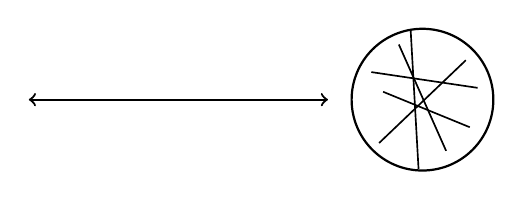
\begin{tikzpicture}[scale=1.0]
\draw[<->, line width=0.8pt] (-3.0,0) -- (0.8,0);
\draw[line width=0.8pt] (2.0,0) circle (0.9);
\draw[line width=0.6pt] (1.45,-0.55) -- (2.55,0.50);
\draw[line width=0.6pt] (1.50,0.10) -- (2.60,-0.35);
\draw[line width=0.6pt] (1.70,0.70) -- (2.30,-0.65);
\draw[line width=0.6pt] (1.35,0.35) -- (2.70,0.15);
\draw[line width=0.6pt] (1.85,0.88) -- (1.95,-0.88);
\end{tikzpicture}
\caption{Clean qualitative reconstruction of the near-horizon sketch.}
\end{figure}

For a macroscopic black hole, much larger than the string scale, this stringy structure is only a small amount of fuzz spread over the horizon. But the lecture immediately asks a sharper question. What happens if the black hole is not much larger than the string scale? What if its Schwarzschild radius becomes comparable to the size of the little string loops that make up the would-be black hole?

That is the point at which the lecture identifies the crossover between the two descriptions.

\section{The Transition Point and the Unfinished Derivation}

The transition point is defined when the Schwarzschild radius becomes comparable to the string length:
\begin{equation}
R_s\sim \ell_s.
\end{equation}
Below that scale it no longer makes sense to insist on a black-hole description. The object simply becomes a string.

\begin{figure}[htbp]
\centering

\includegraphics[width=0.72\textwidth]{lecture_06_figure_05.png}
\caption{Blackboard comparison of black-hole and string entropy formulas. The lower line begins with \(R_s=\); the cleaned transition relation is reconstructed from the surrounding transcript rather than read directly from the frame.}
\end{figure}

The board layout is important here. Susskind places the two entropy formulas one above the other before beginning the transition equation:
\begin{align}
S_{BH} &= \frac{A}{\ell_p^2}=M^2G,\\
S_{ST} &= \frac{L}{\ell_s}=M\ell_s.
\end{align}
These visible equations should be read as scaling statements with suppressed numerical constants. In cleaned notation, the comparison is
\begin{align}
S_{BH} &\sim \frac{A}{\ell_p^2}\sim M^2\ell_p^2,\\
S_{st} &\sim \frac{L}{\ell_s}\sim M\ell_s.
\end{align}

The transition condition can then be rewritten step by step. Since
\begin{equation}
R_s\sim MG_N,
\end{equation}
the condition \(R_s\sim \ell_s\) becomes
\begin{equation}
MG_N\sim \ell_s.
\end{equation}
Using \(G_N=\ell_p^2\), this may be written as
\begin{equation}
M\ell_p^2\sim \ell_s.
\end{equation}
Finally, substituting \(\ell_p=g_s\ell_s\), one finds
\begin{align}
M(g_s^2\ell_s^2) &\sim \ell_s,\\
Mg_s^2\ell_s &\sim 1.
\end{align}
The lecture's spoken algebra in this passage becomes rather messy, so this cleaned reconstruction should be understood as a cautious standard form of what is being derived.

The lecture then supplies the last logical ingredient. If a control parameter is changed adiabatically, that is, slowly enough, then the entropy does not change. In the present application one simply writes
\begin{equation}
\Delta S=0
\end{equation}
for an adiabatic variation of \(g_s\). This is the step that finally explains why the long detour through strings is relevant to the entropy of black holes at all.

The strategy now becomes transparent:
\begin{enumerate}
\item Start with a black hole of mass \(M_0\) at some coupling \(g_{s,0}\).
\item Decrease the coupling adiabatically.
\item At the transition point the object becomes a string.
\item Use the string description to compute the entropy there.
\item Because the entropy did not change during the adiabatic evolution, identify that string entropy with the entropy of the original black hole.
\end{enumerate}
This is exactly where the lecture stops. The pieces have all been laid out, but the final assembly is deferred. Susskind's point is that one does not need a complicated formal derivation with integrals and differential equations; what one needs is the right chain of physical identifications.

\section{Summary}

The lecture unfolds as a single argument. Entropy is first reinterpreted as hidden microscopic information. The black-hole entropy problem is then put on the same footing as the entropy of an ordinary fluid: the thermodynamic statement is clear, but the microscopic carriers are not. String theory supplies the basic scales \(\ell_s\) and \(g_s\), and dimensional analysis together with the exchange-picture analogy yields
\begin{equation}
\ell_p^2=G_N,
\qquad
\ell_p=g_s\ell_s.
\end{equation}
With those relations in hand, the lecture places two formulas side by side,
\begin{equation}
S_{BH}\sim M^2\ell_p^2,
\qquad
S_{st}\sim M\ell_s,
\end{equation}
and uses their mismatch to motivate the coupling-dial thought experiment. A long string at weak coupling contracts as gravity is turned on, becomes a black hole when its size falls below its Schwarzschild radius, and is seen from the outside as stringy structure living on or near the horizon. The crossover occurs when
\begin{equation}
R_s\sim \ell_s,
\qquad
Mg_s^2\ell_s\sim 1.
\end{equation}
The final step is adiabatic invariance of entropy. That principle is what allows the string entropy at the transition point to be carried back to the original black hole. The lecture does not complete the derivation here; instead it ends by making the logic of the derivation visible.